%In this section, the method chosen to perform simulations for both the top and stop decays are shown. In addition, the preparation of data is explained in order to jusitfy the usage of ML and their results.\\
%-------------------------------------------------------------------------%
\section{Background and Signal of interest}
As discussed in Section \ref{sec:Sims}, MadGraph5 is the chosen software to perform particle collider simulations, in which one million events were produced for both the signal and background events. At the generator level, in order to meet the pre-selection criteria listed in the following subsection, we limit the missing transverse energy $\cancel{\it{E}}_{T}$ to a minimum of 200 GeV as the signatures significantly differ between our signal and backgrounds as seen in Figure \ref{fig:topMET}. The difference in MET affects the results upon building the classifiers and efficiencies, thus by requiring the signatures to be in a similar range we can observe the efficiency in our results in a reasonable range. In addition, MG5 calculates a cross-section value associated to each process generated, also required for our analysis. \\

\begin{figure}[htbp]
    \centering
    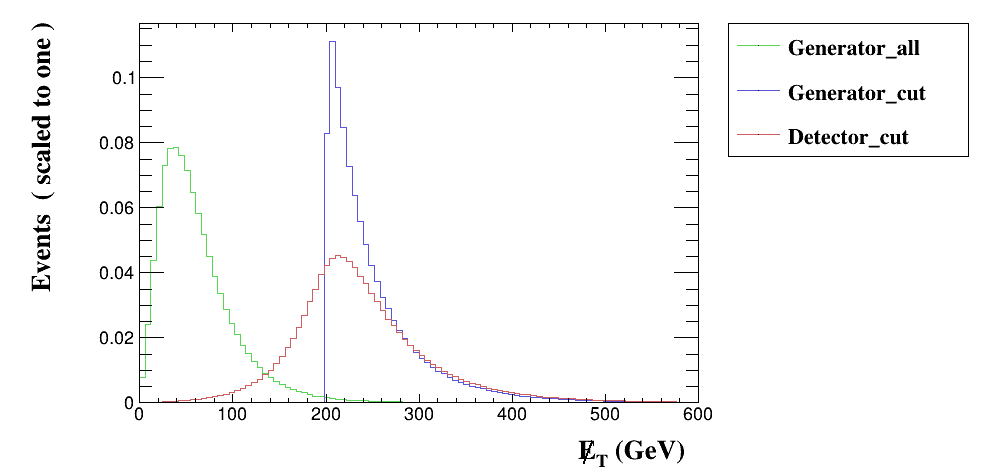
\includegraphics[width=0.75\linewidth]{top-MET.png}
    \caption{A histogram to depict the variation in generator-level and detector-level simulation in the top quark production $pp \rightarrow t\Bar{t} \rightarrow bW^{-}\Bar{b}W^{+} \rightarrow l^{\pm}\nu_l(\Bar{\nu}_l)q\Bar{q}$.}
    \label{fig:topMET}
\end{figure}

Since the decay process involves both leptonic and hadronic particles as seen in Figure \ref{fig:topdecay}, the following were defined in order to make the simulation complete. \\

\begin{lstlisting}[mathescape = true]
        define leptonic = l+ l- ta+ ta- vl vl$\sim$
        define hadronic = u c d s u$\sim$ c$\sim$ d$\sim$ s$\sim$ b b$\sim$
\end{lstlisting}

For the background process defined by Equation (\ref{eq:background}), the command to generate the events is given by
\begin{lstlisting}[mathescape = true]
            generate p p > t t$\sim$ , 
            (t > W+ b , W+ > leptonic leptonic), 
            (t$\sim$ > W- b$\sim$, W- > hadronic hadronic)
        
            add process p p > t1 t1$\sim$ ,
            (t > W+ b , W+ > hadronic hadronic), 
            (t$\sim$ > W- b$\sim$, W- > leptonic leptonic)
\end{lstlisting}
where a diagram from one of its generated events can be seen in Figure \ref{fig:bkrdFeyn}. \\

Similarly, the process for signal production follows that of Equation (\ref{eq:signal}), in which the command for generating the events is given by
\begin{lstlisting}[mathescape = true]
        generate p p > t1 t1$\sim$ ,
        (t1 > t n1, (t > W+ b , W+ > leptonic leptonic)),
        (t1~ > t$\sim$ n1, (t$\sim$ > W- b$\sim$, W- > hadronic hadronic))
        
        add process p p > t1 t1$\sim$ , 
        (t1 > t n1, (t > W+ b , W+ > hadronic hadronic)), 
        (t1$\sim$ > t$\sim$ n1, (t$\sim$ > W- b$\sim$, W- > leptonic leptonic))
\end{lstlisting}
with an accompanying example diagram given in Figure \ref{fig:sigFeyn}. \\

\noindent\begin{minipage}{\textwidth}
\centering
  \begin{minipage}[htbp]{0.45\textwidth}
    \centering
    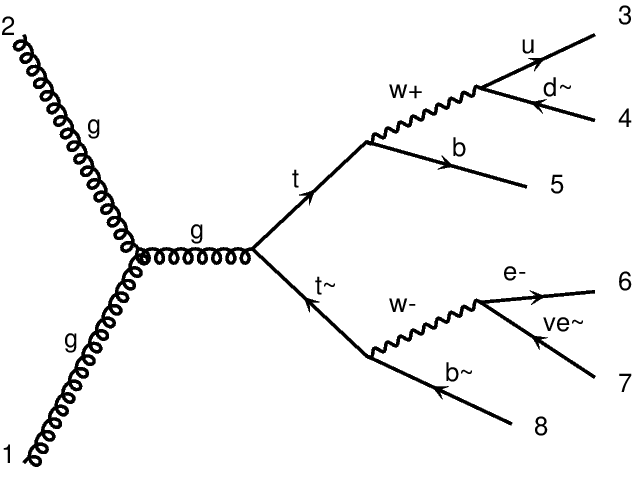
\includegraphics[width=\linewidth, keepaspectratio=true]{top_MG5.png}
    \captionof{figure}{Feynman diagram of the leading order background process $pp \rightarrow t \Bar{t} \rightarrow b\Bar{b}l^{+}jj\cancel{\it{E}}_{T} $.}
    \label{fig:bkrdFeyn}
  \end{minipage}
  %\hfill
  \begin{minipage}[htbp]{0.45\textwidth}
    \centering
    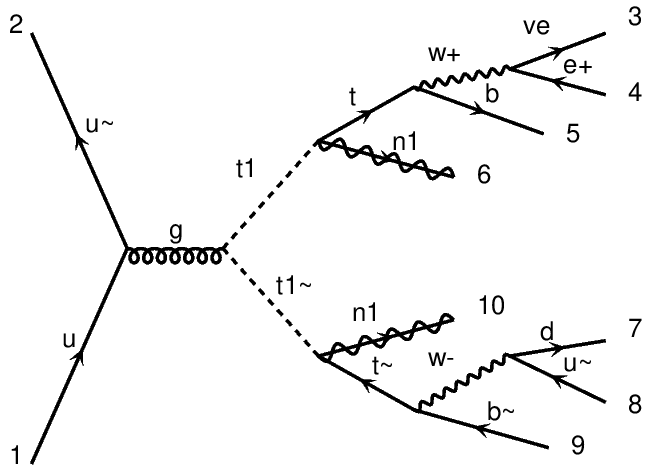
\includegraphics[width=\linewidth, keepaspectratio=true]{stop_MG5.png}
    \captionof{figure}{Feynman diagram of the leading order signal process $ pp \rightarrow \Tilde{t}\Tilde{t^*} \rightarrow t \Bar{t} \chi^0_1\chi^0_1 \rightarrow b\Bar{b}l^{+}jj\cancel{\it{E}}_{T} $ where the final states are identical to that of the background in Figure \ref{fig:bkrdFeyn}.}
    \label{fig:sigFeyn}
  \end{minipage}
\end{minipage}
%-------------------------------------------------------------------------%
\section{Preselection}

During the pre-selection process we require three conditions the data must meet, based on several. 
\begin{itemize}
    \item $\cancel{\it{E}}_{T}>250$ GeV
    \item Only one charged lepton (No sign discrimination)
    \item A minimum of one $b$-tagged jet. The highest $b$-tagged jet is considered the only $b$-jet and the rest are considered ordinary jets.\\
\end{itemize}

Table \ref{tab:benchmarks} depicts the number of events remaining after each pre-selection criteria applied, from left to right. The disparity in the initial events comes from the fact that we require an equal amount of data in the final count in order to have a 50:50 split between the signal and background events in our data. This allows our classifier to be built effectively. In adition, Table \ref{tab:benchmarks} lists the cross-section, $\sigma$, of each process simulated, which will be useful as will be discussed in the next section. \\

\begin{table}[htbp]
    \centering
    \begin{tabular}{c|c|c|c|c||c} 
    \toprule
    Data & Initial & $\cancel{\it{E}}_{T}>250$ GeV & $1l^\pm$ & $\min(1b)$ & Cross-section, $\sigma$ (pb) \\
    \midrule
    \rowcolor{gray!6} Benchmark1 & 776800 & 559371 & 179472 & 101488 & $1.6\times10^{-4} \pm 6.7\times10^{-8}$ \\
    Benchmark2 & 758458 & 611119 & 187179 & 101488 & $4.0\times10^{-4} \pm  5.4\times10^{-7}$ \\
    \rowcolor{gray!6} Benchmark3 & 758498 & 643458 & 191944 & 101488 & $6.6\times10^{-4} \pm 2.7\times10^{-7}$ \\
    Benchmark4 & 818636 & 515694 & 172171 &101488  & $4.0\times10^{-3} \pm 1.6\times10^{-6}$ \\
    \rowcolor{gray!6} Background & $10^6$ & 357273 & 123933 & 101488 & $2.5 \pm 1.3\times10^{-3}$ \\
    \bottomrule
    \end{tabular}
    \caption{The number of events remaining at each step of the pre-selection process.} 
    \label{tab:preselection}
\end{table}